\documentclass[11pt]{beamer}
\usetheme{CambridgeUS}
\usepackage[utf8]{inputenc}
\usepackage[german]{babel}
\usepackage[T1]{fontenc}
\usepackage{amsmath}
\usepackage{amsfonts}
\usepackage{amssymb}
\usepackage{tikz}
\usepackage{enumitem}
\usepackage{subfigure}

\usetikzlibrary{positioning,shapes.geometric}


\author{Hannes Benne}
\title{Automatische Schnitterkennung in Videos}
%\setbeamercovered{transparent} 
%\setbeamertemplate{navigation symbols}{} 
%\logo{} 
%\institute{} 
%\date{} 
%\subject{} 
\begin{document}
\setlist[itemize,1]{label=$\triangleright$}
\begin{frame}
\titlepage
\end{frame}

%\begin{frame}
%\tableofcontents
%\end{frame}

\begin{frame}{Warum geht es?}
\begin{itemize}
\item In Videos sollen automatisch Szenen bzw. Übergänge zwischen verschiedenen Szenen erkannt werden.
\item Motivation: Einfache Nachbearbeitung von Videos.
\item Klassifizierung von Frames $\rightarrow$ Aktuelle Szene | Neue Szene
\end{itemize}
\end{frame}

\begin{frame}{Automatische Schnitterkennung}
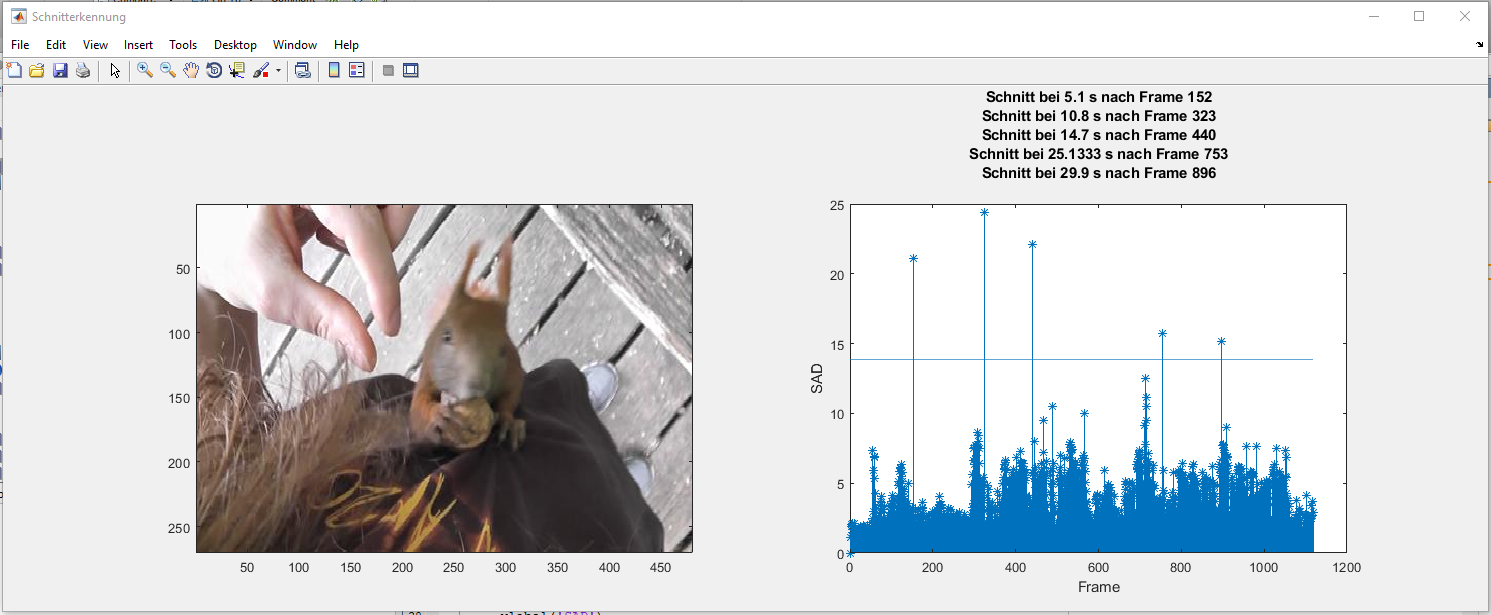
\includegraphics[scale=0.31]{sadstem2.png}
\end{frame}

\begin{frame}[t]{Signalerfassung}
Videoaufnahmen von verschiedenen Tieren in Volkspark Hasenheide:
\begin{figure}
	\centering
	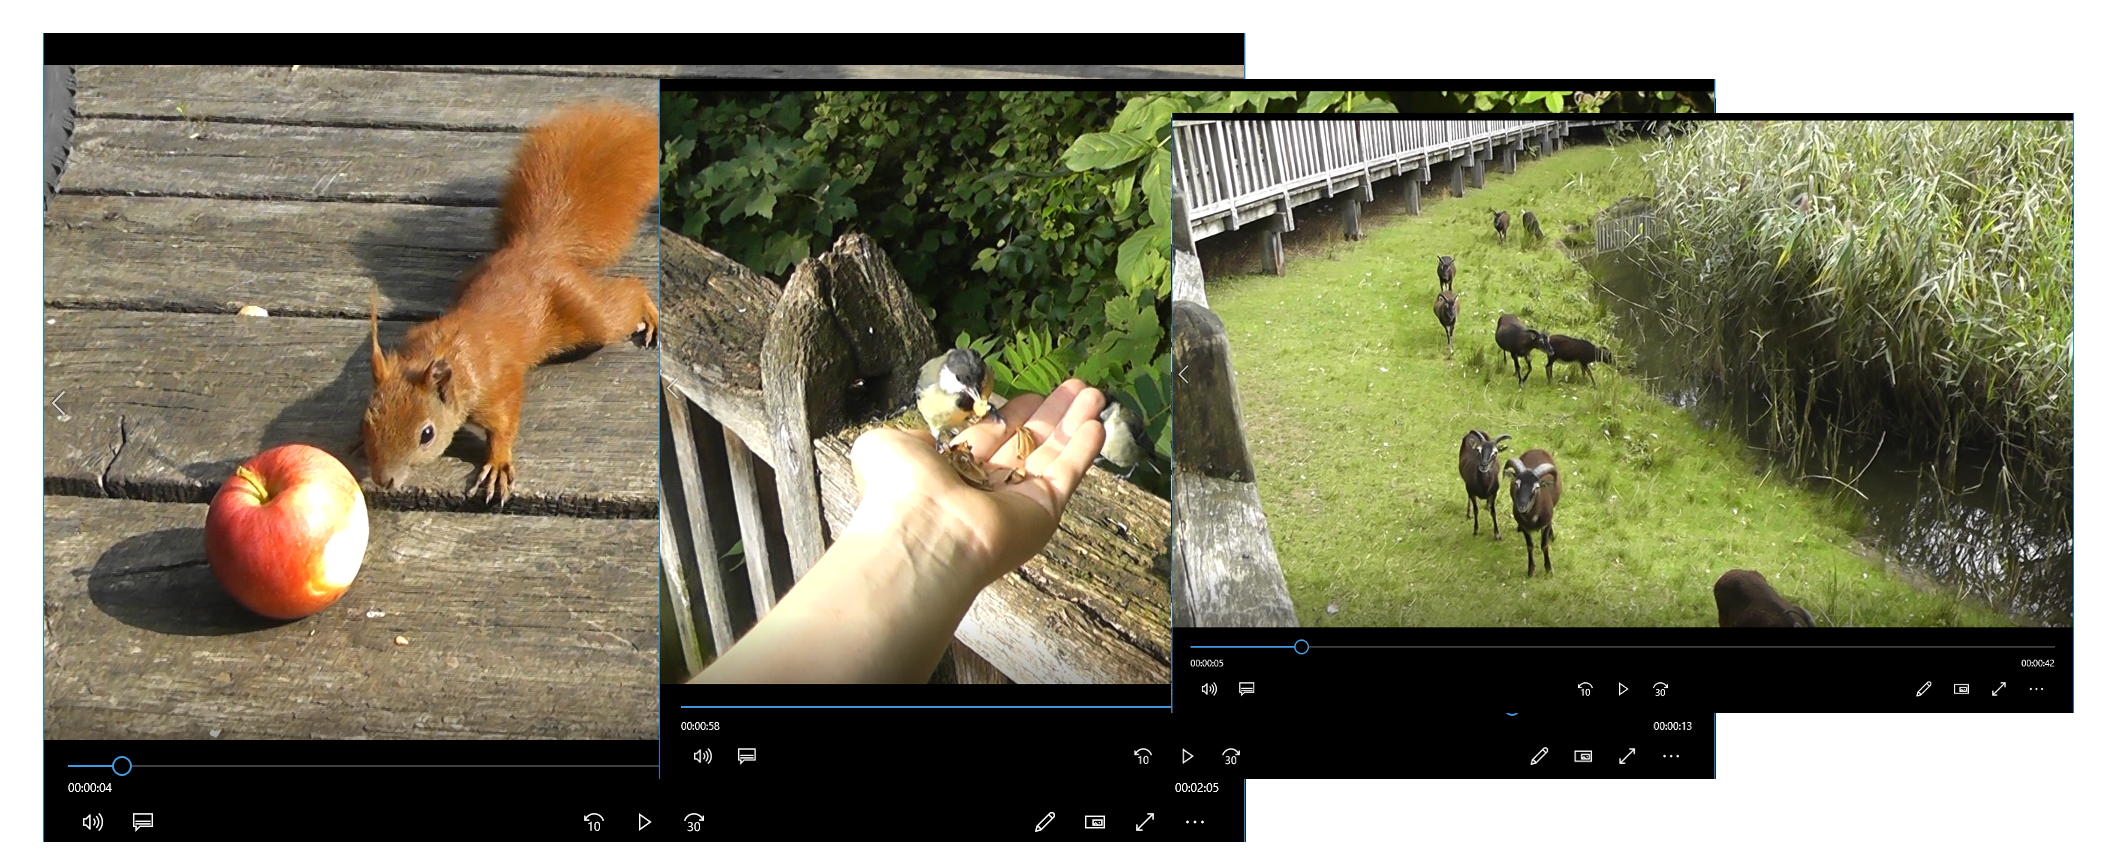
\includegraphics[scale=0.15]{Signalerfassung}
\end{figure}
\end{frame}

\begin{frame}{Vorverarbeitung}
\begin{itemize}
\item Bildgröße verringern von 1920 px $\times$ 1080 px auf 480 px $\times$ 270 px  \\
$\rightarrow$ weniger Rechenaufwand. 
\item Transformation in YCbCr Farbraum oder in Graustufenbild. 
\end{itemize} 
~\newline
~\newline
\end{frame}

\begin{frame}{Merkmalsgewinnung}
Suchen eine Metrik dafür, wie ähnlich zwei Bilder zueinander sind.
\begin{itemize}
\item Summe der absoluten Differenzen (SAD)
\item Histogramm-Differenz (HD)
\item  Edge Change Ratio (ECR)
\end{itemize}
Summe der absoluten Differenzen liefert die besten Ergebnisse: https://docplayer.org/53107729-2-schnitterkennung-videoanalyse.html
\end{frame}


\begin{frame}{Summe der absoluten Differenzen}
Eingabe: Zwei gleich große Bilder $B_1, B_2$. 
\[ SAD = \dfrac{1}{b\cdot h}\sum_{x=0}^{b-1} \sum_{y=0}^{h-1} | B_2(x,y) - B_1(x,y) | \]

Farbbilder entweder in Graustufen umwandeln oder (empfohlen) nur Y - Komponente verwenden. 
\end{frame}

\begin{frame}{Summe der absoluten Differenzen}
\begin{figure}
    \subfigure[Frame 83]{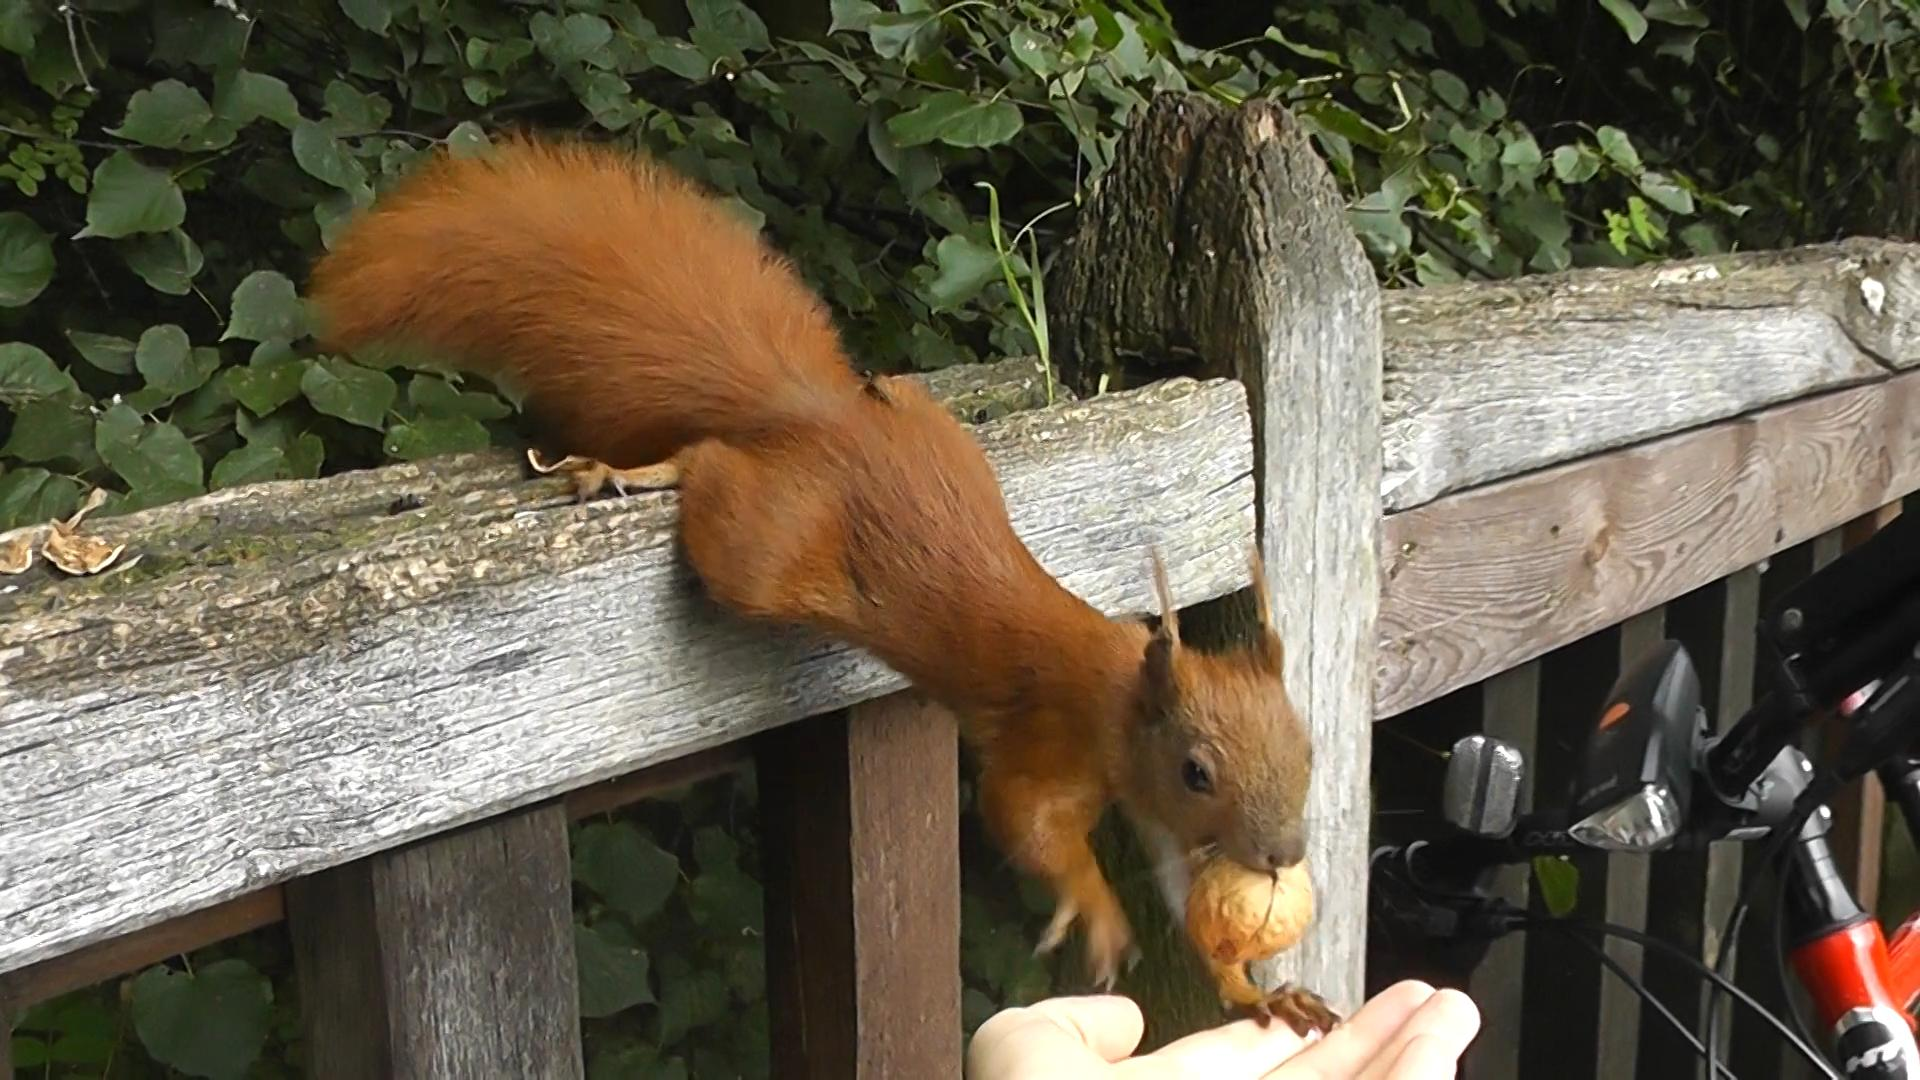
\includegraphics[width=0.49\textwidth]{frame83.jpg}} 
    \subfigure[Frame 84]{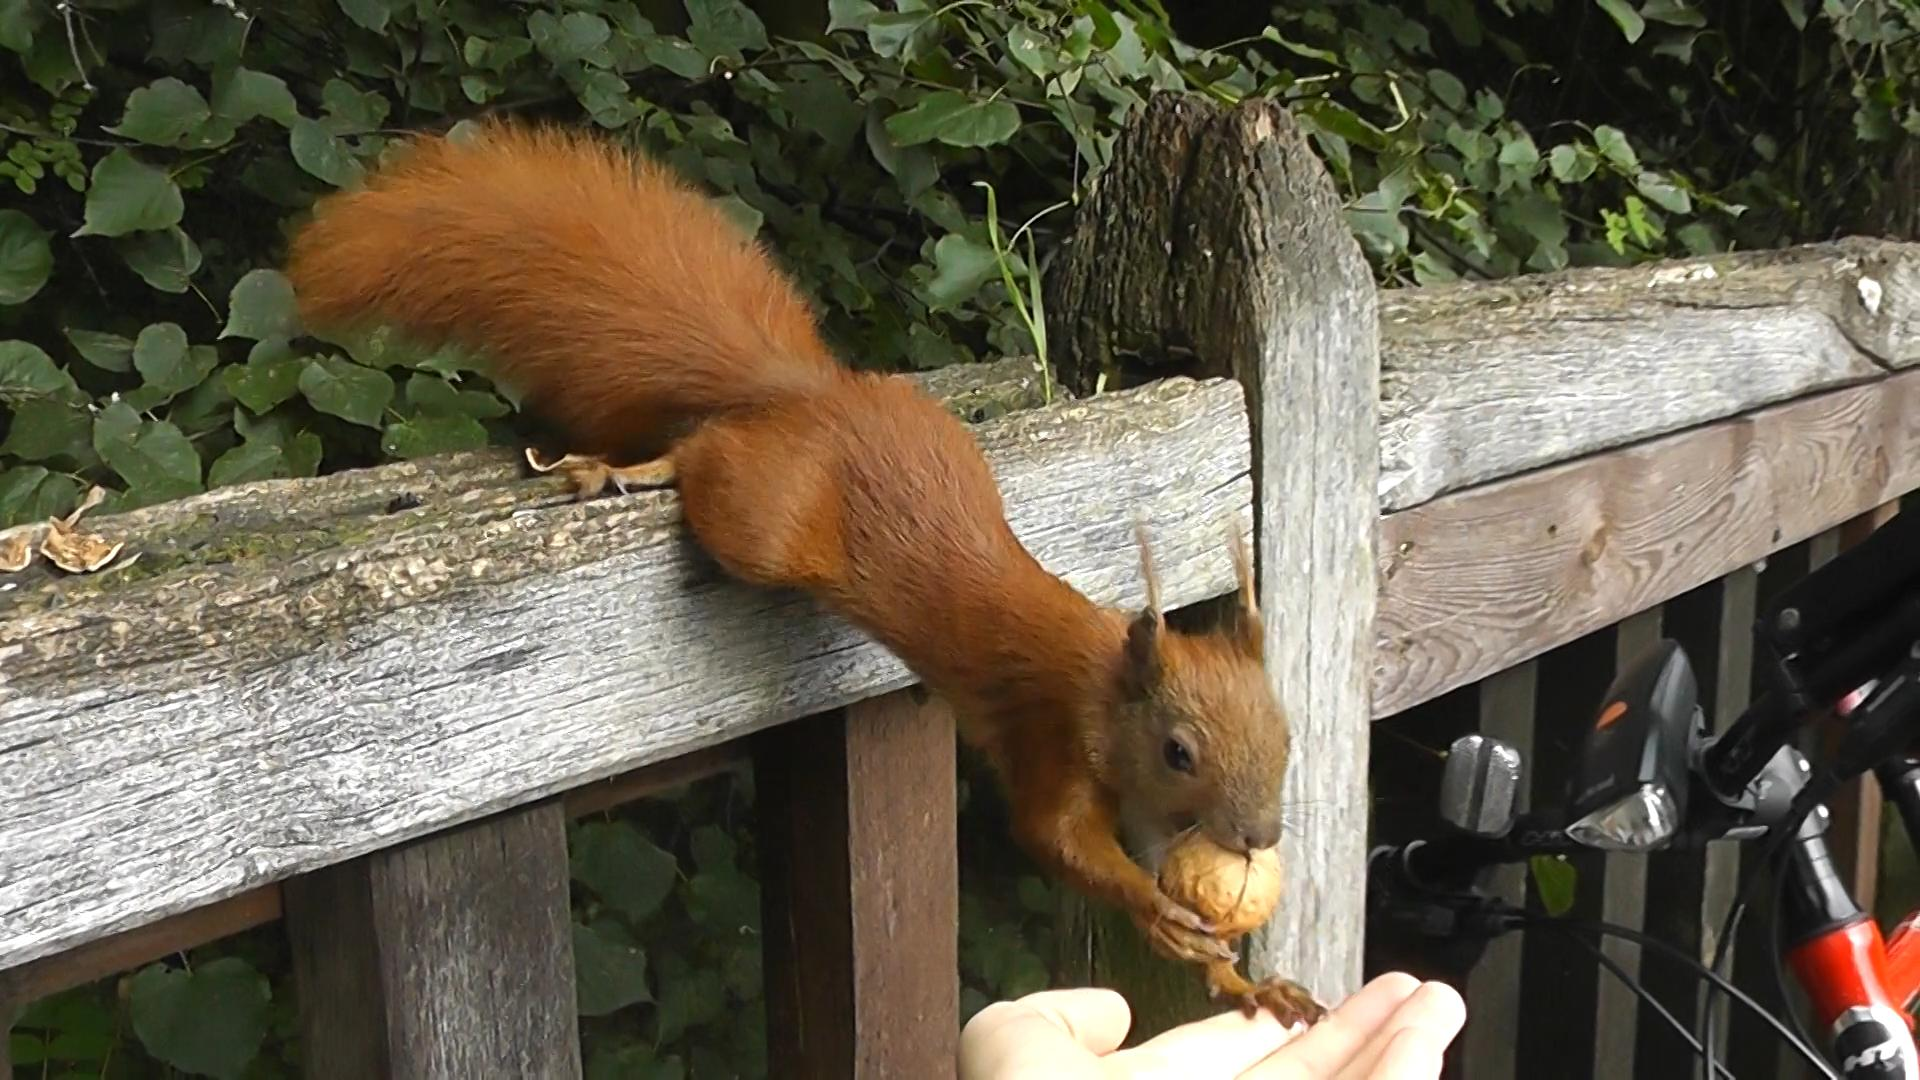
\includegraphics[width=0.49\textwidth]{frame84.jpg}} 
\caption{Aufeinanderfolgende Frames der gleiche Szene. $SAD = 3.3445$} 
\end{figure} 
\end{frame}

\begin{frame}{Summe der absoluten Differenzen}
\begin{figure}
    \subfigure[Frame 322]{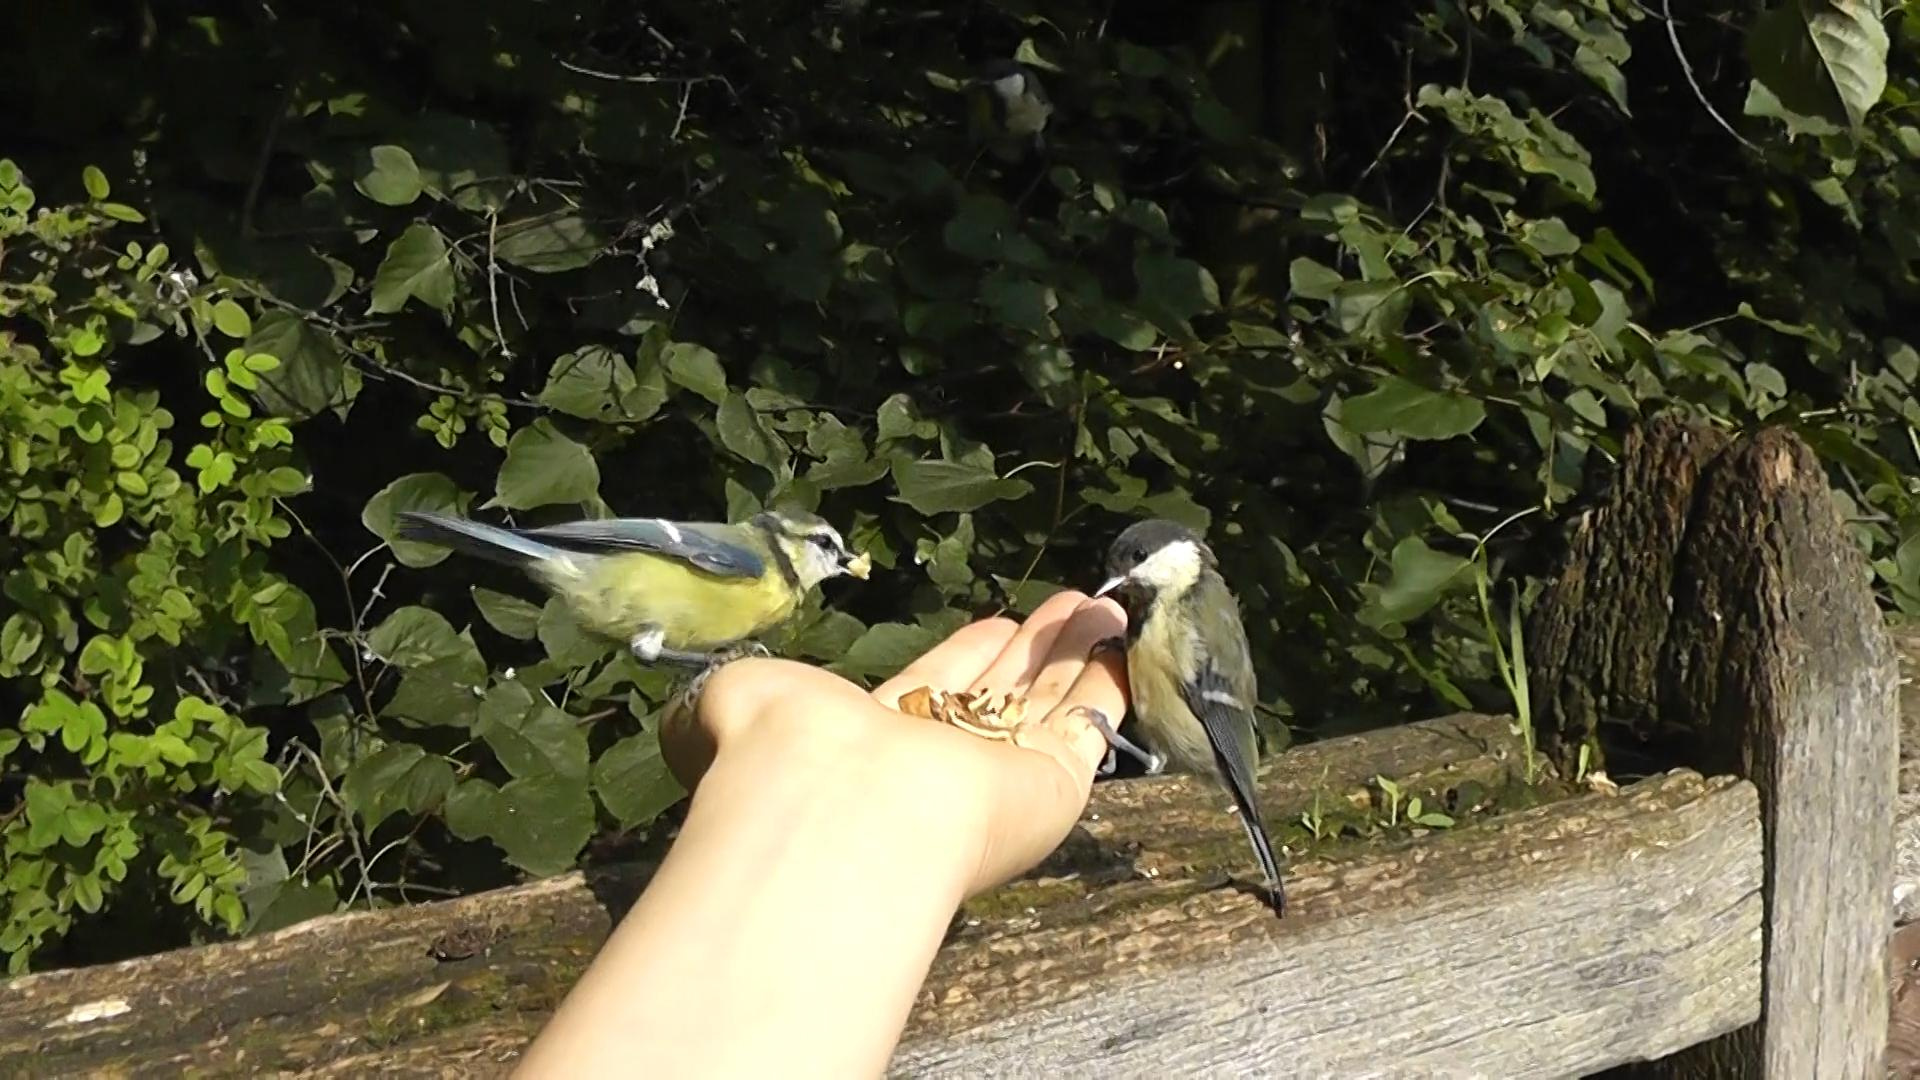
\includegraphics[width=0.49\textwidth]{frame322.jpg}} 
    \subfigure[Frame 755]{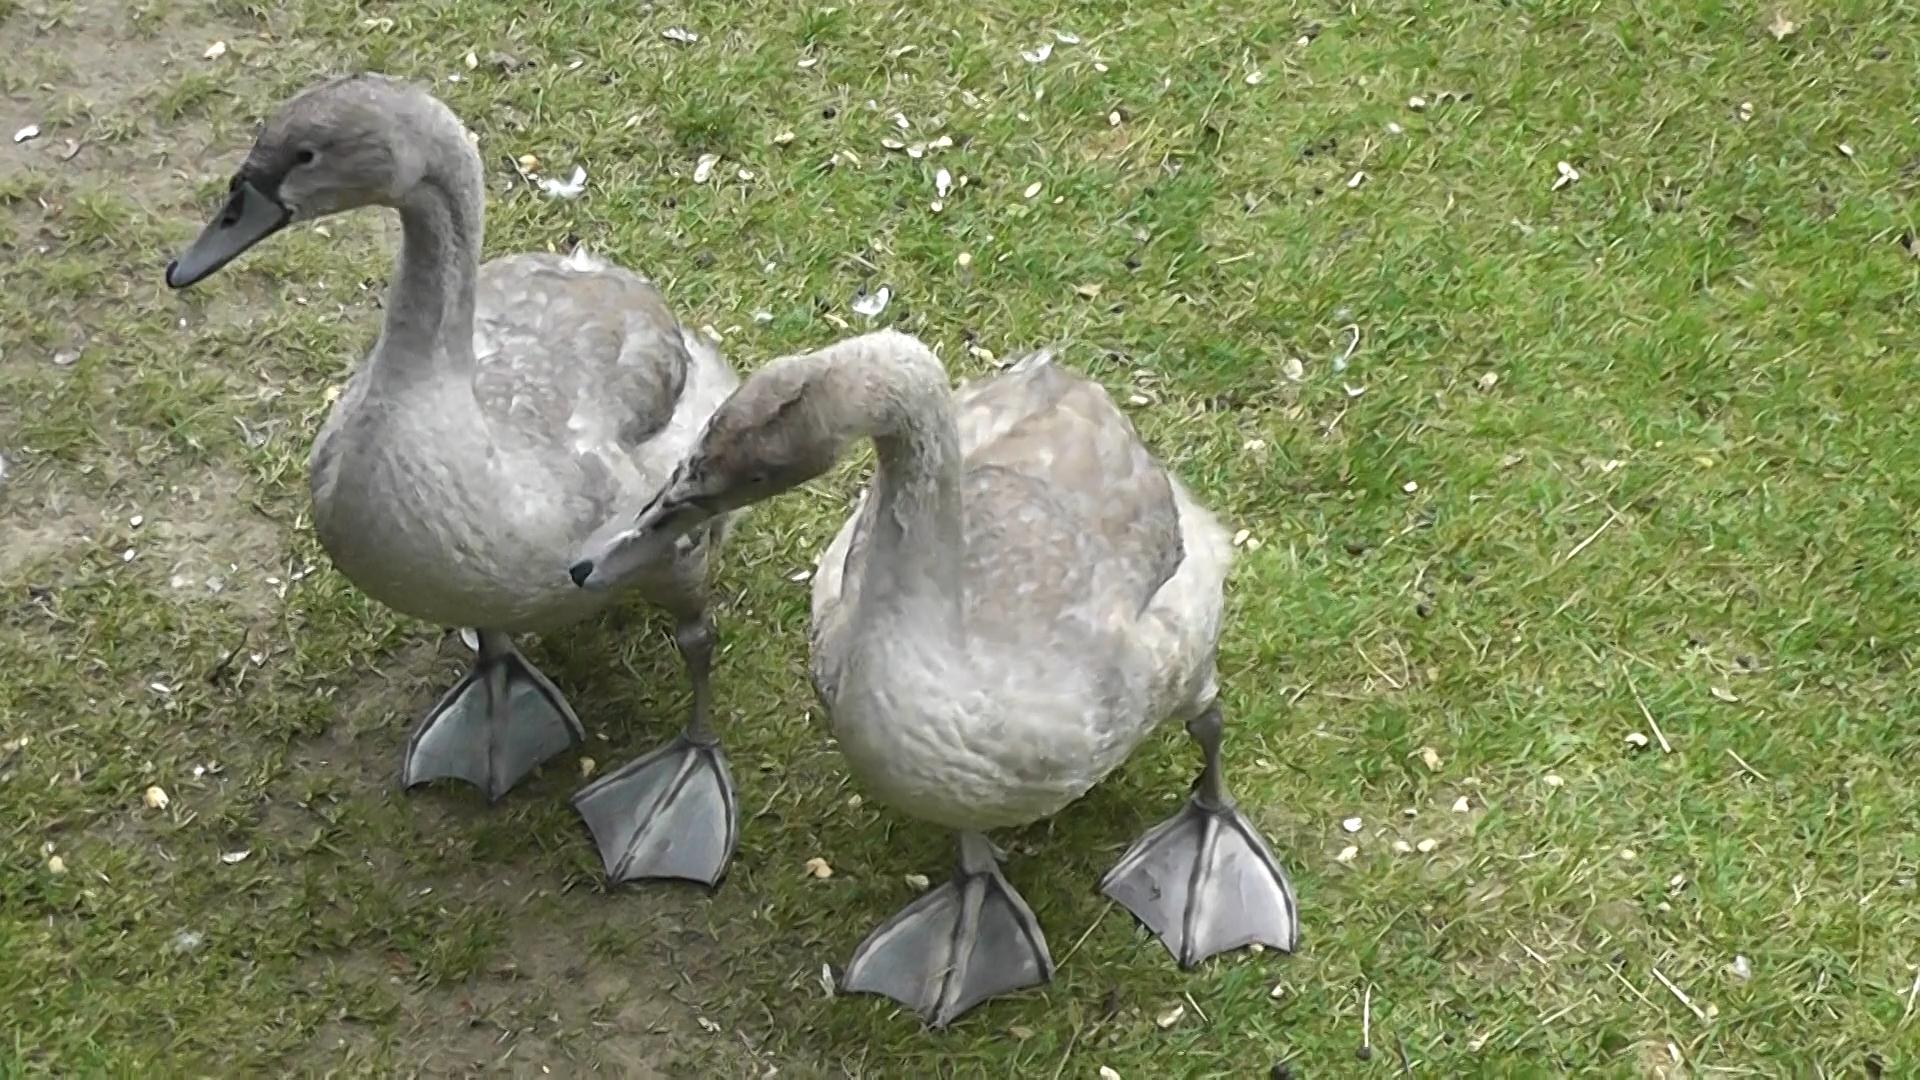
\includegraphics[width=0.49\textwidth]{frame775.jpg}} 
\caption{Frames aus unterschiedlichen Szenen. $SAD = 24.585$} 
\end{figure} 
\end{frame}

\begin{frame}{Summe der absoluten Differenzen}
\begin{figure}
    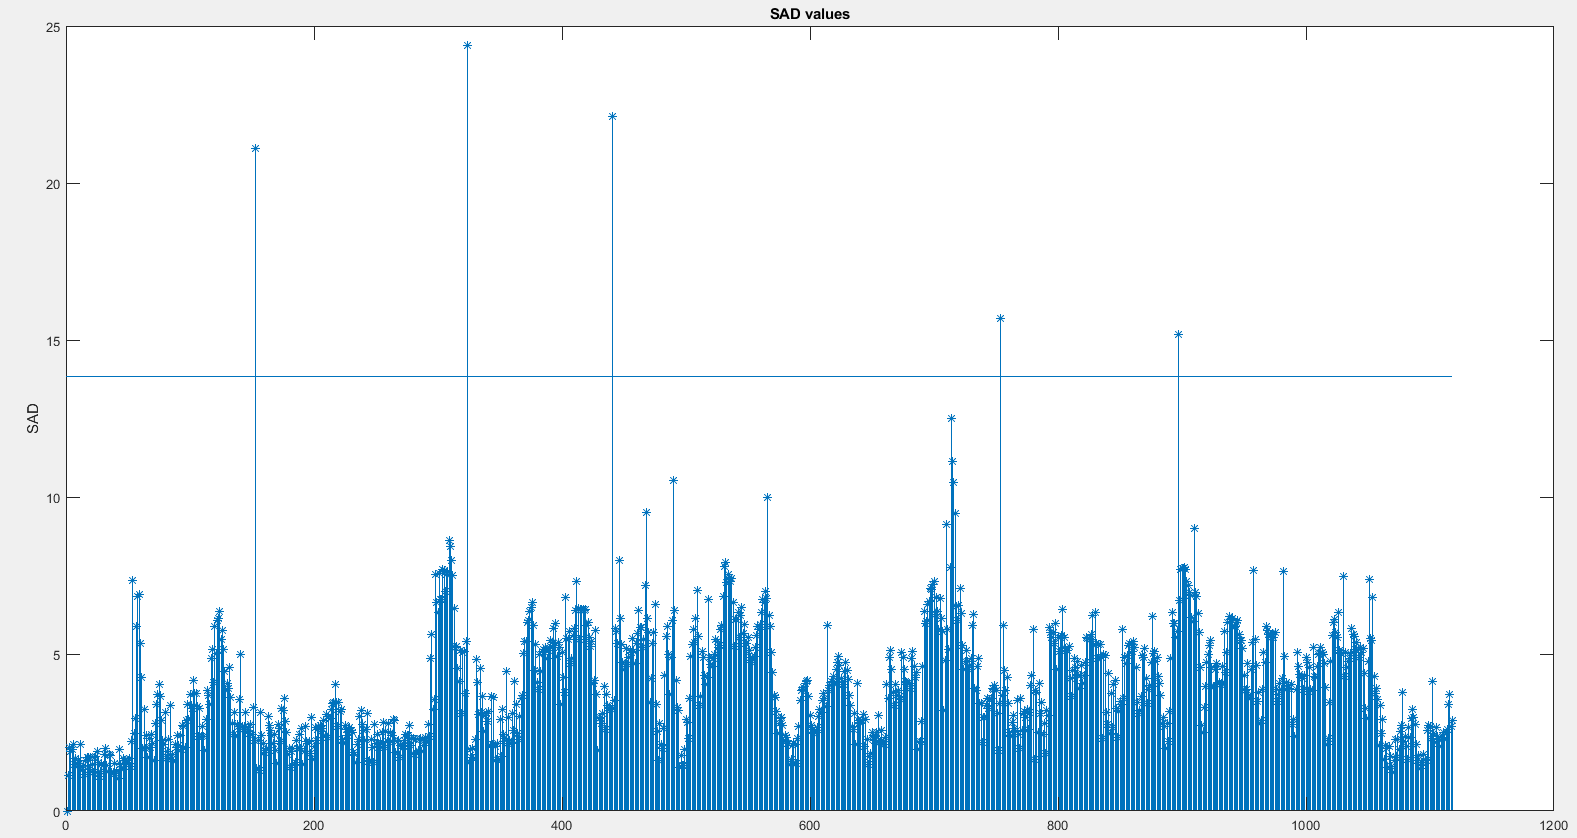
\includegraphics[scale=0.3]{sadstem.png} 
\end{figure} 
\end{frame}

\begin{frame}{Summe der absoluten Differenzen}
\begin{figure}
    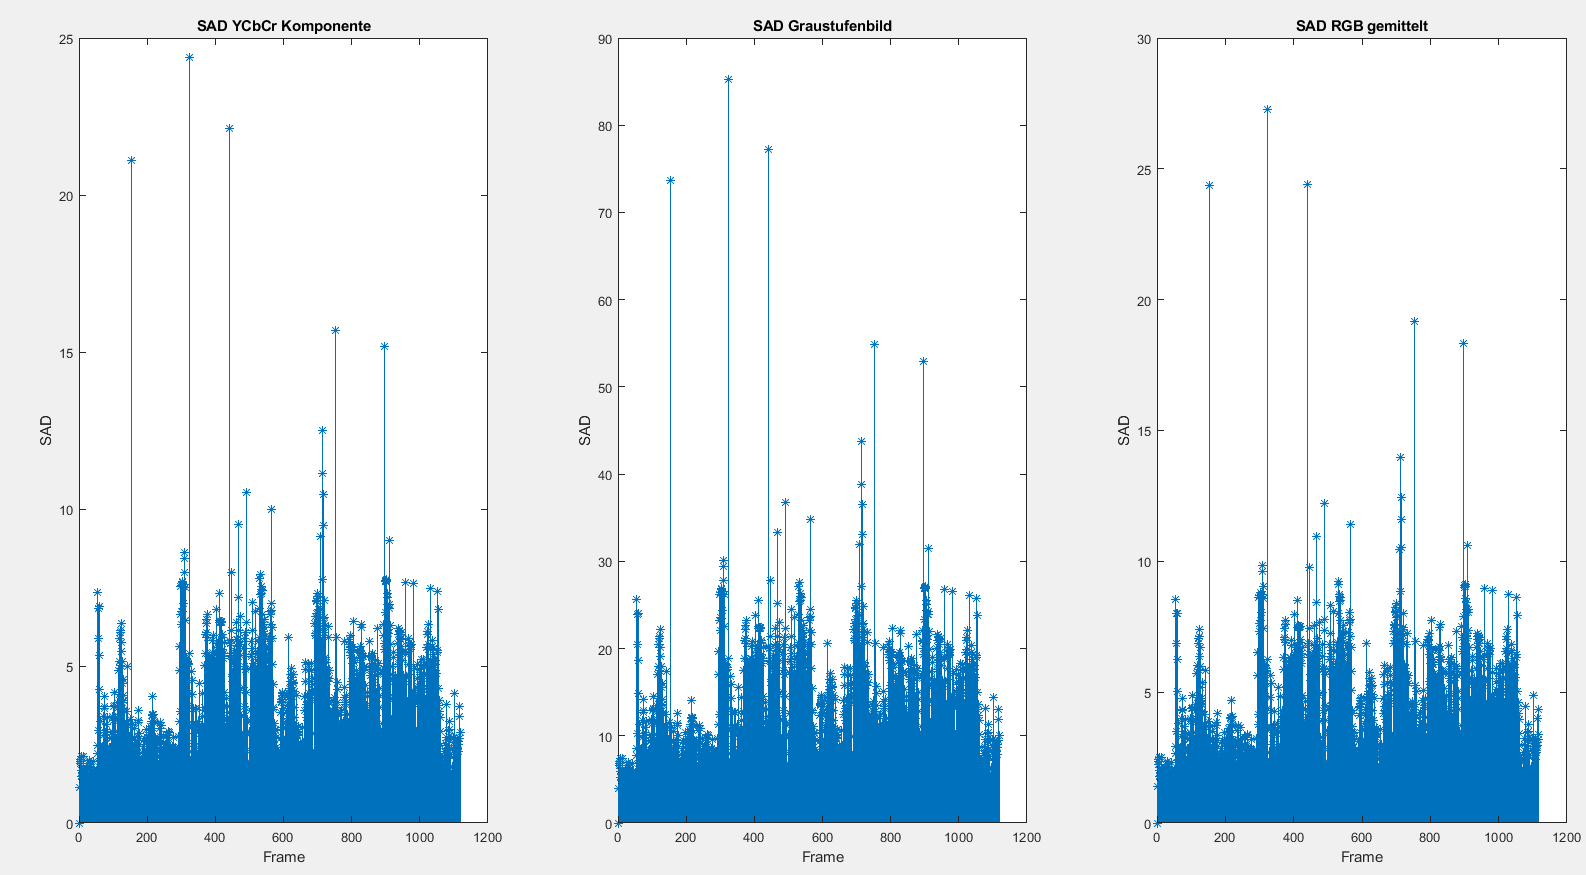
\includegraphics[scale=0.3]{sadstem3.png} 
\end{figure} 
\end{frame}

\begin{frame}{Klassifikation}
Für jedes Bild den $SAD$--Wert mit einem Schwellwert $S$ vergleichen.\\
Wenn $SAD < S$ $\rightarrow$ Bild gehört nicht zu einer neuen Szene/ kein Schnitt im Video\\  
Wenn $SAD \geq S$ $\rightarrow$ Bild gehört  neuen Szene/Schnitt im Video\\  
$S$ wird aus Trainingsdaten bestimmt. Mittelwert aus kleinstem $SAD$ - Wert der Schnittframes und größtem $SAD$-Wert der nicht Schnittframes.
\end{frame}

\begin{frame}{Klassifikation}
Projektion der SAD Werte auf die y-Achse.
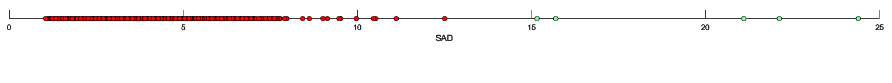
\includegraphics[scale=0.5]{SADProjektion.png}
\end{frame}

\begin{frame}{Varianzanalyse}
$H_0:$ Das Merkmal SAD zum Vorgängerbild ist nicht geeignet um die Klassen \glqq aktuelle Szene\grqq{} und \glqq neue Szene\grqq{} voneinander zu trennen. \\
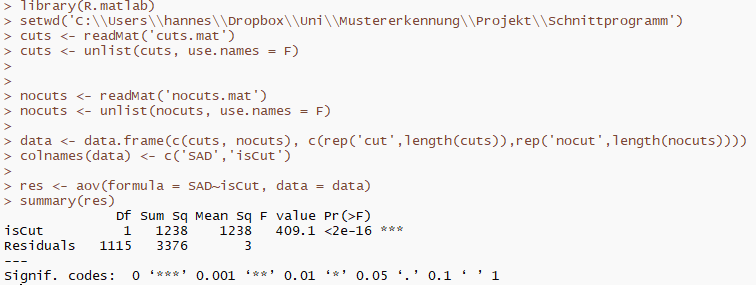
\includegraphics[scale=0.44]{statistik.png}\\
$p < 0.5$, also lehnen wir $H_0$ ab.
\end{frame}

\begin{frame}{Bewertung der Klassifikation}
C: korrekt erkannte Schnitte.\\
F: fehlerhaft erkannte Schnitte\\
M: nicht erkannte Schnitt\\
Präzision: Alle erkannten Schnitte sind echte Schnitte.
\[ P = \frac{C}{C+F} \in [0,1] \] 
Vollständigkeit: In der Menge der erkannten Schnitte sind alle Schnitte enthalten.
\[ V = \frac{C}{C+M} \in [0,1] \]
Kombination aus Präzision und Vollständigkeit.
\[ F_1 = 2 \cdot \frac{P\cdot V}{P + V} \in [0,1] \]
In meinen Testdaten war: $F_1 = 1$. 

\end{frame}

\end{document}

